\chapter{Software Testing}
\label{ch:testing}

Testing is the primary defence against defects escaping to users. Yet testing cannot prove the absence of bugs---it can only increase confidence. This chapter organises testing by level, introduces test-driven development, and explains how coverage guides (but does not guarantee) quality.

\section{Why Test?}

Every defect has a cost that grows with time-to-detection. Requirements bugs found in production can cost $100\times$ more than those caught in review. Testing shifts detection earlier. Two complementary perspectives frame the activity:

\begin{itemize}
    \item \textbf{Verification} --- are we building the product right? (does code meet spec?)
    \item \textbf{Validation} --- are we building the right product? (does spec meet user need?)
\end{itemize}

Testing also includes \emph{debugging} (finding and fixing the cause after a failure is observed) and \emph{quality assurance} (process measures that prevent defects).

\section{Levels of Testing}

\begin{figure}[h]
\centering
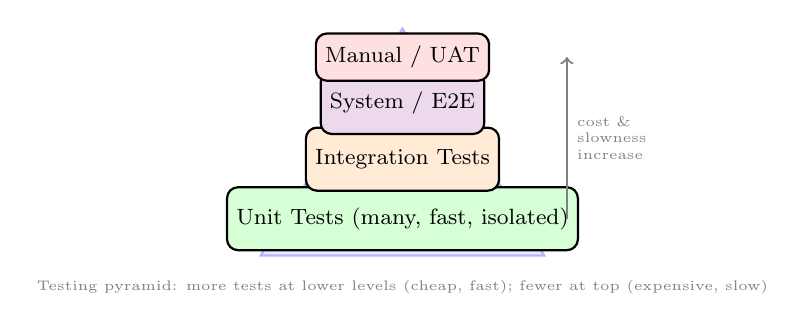
\begin{tikzpicture}[scale=0.72, every node/.style={font=\footnotesize}]
  \draw[fill=blue!8,draw=blue!30,thick] (0,0) -- (5,0) -- (2.5,4.0) -- cycle;
  \node[draw,fill=green!16,rounded corners,minimum width=3.0cm,minimum height=0.8cm,thick] at (2.5,0.65) {Unit Tests (many, fast, isolated)};
  \node[draw,fill=orange!16,rounded corners,minimum width=2.4cm,minimum height=0.8cm,thick] at (2.5,1.7) {Integration Tests};
  \node[draw,fill=violet!15,rounded corners,minimum width=1.8cm,minimum height=0.8cm,thick] at (2.5,2.7) {System / E2E};
  \node[draw,fill=red!12,rounded corners,minimum width=1.1cm,minimum height=0.6cm,thick] at (2.5,3.5) {Manual / UAT};
  \node[font=\tiny,gray,align=center] at (2.5,-0.55) {Testing pyramid: more tests at lower levels (cheap, fast); fewer at top (expensive, slow)};
  \draw[->,thick,gray] (5.4,0.65) -- (5.4,3.5) node[midway,right,font=\tiny,align=left] {cost \&\\slowness\\increase};
\end{tikzpicture}
\caption{Testing pyramid -- the foundation is many fast unit tests; integration and system tests are fewer and more expensive. An inverted ``ice-cream cone'' (many E2E tests) is an anti-pattern.}
\end{figure}

\begin{itemize}
    \item \textbf{Unit testing} --- tests a single class/method in isolation, with dependencies mocked or stubbed. Fast (milliseconds), precise failure localisation.
    \item \textbf{Integration testing} --- verifies interactions between units: does module~A call module~B correctly? Catches interface mismatches and contract violations. Subsumes component and subsystem integration.
    \item \textbf{System testing} --- validates the assembled system against requirements in an environment resembling production. Includes functional and non-functional (performance, security, usability) testing.
    \item \textbf{Acceptance testing (UAT)} --- customer-facing validation that the system meets business needs; often manual and scenario-based.
\end{itemize}

A balanced portfolio respects the pyramid shape: roughly $70\%$ unit, $20\%$ integration, $10\%$ system/E2E by count, with execution time dominated by the lower levels.

\section{Test Design Techniques}

\subsection{Black-Box Techniques}

Design tests from the specification without looking at code:

\begin{itemize}
    \item \textbf{Equivalence partitioning} --- divide inputs into classes expected to behave the same; test one representative per class plus boundaries.
    \item \textbf{Boundary-value analysis} --- errors cluster at edges; test at \texttt{min}, \texttt{min+1}, \texttt{max-1}, \texttt{max}.
    \item \textbf{Decision tables} --- enumerate combinations of conditions and expected actions.
\end{itemize}

\subsection{White-Box Techniques}

Design tests from code structure: \emph{statement coverage} (every line executed), \emph{branch coverage} (every branch taken both ways), \emph{path coverage} (every path exercised, often infeasible). Branch coverage subsumes statement coverage; path coverage subsumes branch.

\begin{lstlisting}[language=Java,caption={Branch coverage: two tests cover both branches.}]
boolean isEligible(int age, boolean isMember) {
    if (age >= 18 && isMember) return true; // branch 1
    return false;                            // branch 2
}
// Test 1: isEligible(20, true)  -> true  (covers then-branch)
// Test 2: isEligible(16, false) -> false (covers else-branch)
// Branch coverage = 100%, but is it sufficient? Consider (20,false).
\end{lstlisting}

\section{Test-Driven Development (TDD)}

TDD inverts the usual order: write a failing test first (red), write minimal code to pass (green), then refactor with tests as a safety net. The cycle is deliberately short (minutes).

\begin{figure}[h]
\centering
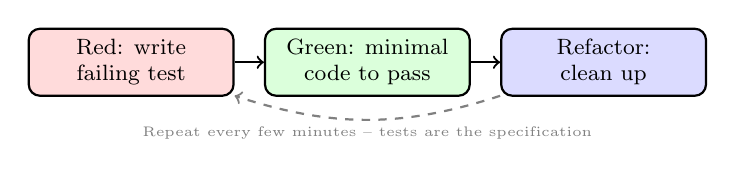
\begin{tikzpicture}[scale=0.75, every node/.style={font=\footnotesize}]
  \tikzstyle{mystep}=[draw,rounded corners,minimum width=2.6cm,minimum height=0.85cm,align=center,thick]
  \node[mystep,fill=red!14] (r) at (0,0) {Red: write\\failing test};
  \node[mystep,fill=green!14] (g) at (4,0) {Green: minimal\\code to pass};
  \node[mystep,fill=blue!14] (refnode) at (8,0) {Refactor:\\clean up};
  \draw[->,thick] (r) -- (g);
  \draw[->,thick] (g) -- (refnode);
  \draw[->,thick,dashed,gray,bend left=18] (refnode) to (r);
  \node[font=\tiny,gray,align=center] at (4,-1.2) {Repeat every few minutes -- tests are the specification};
\end{tikzpicture}
\caption{TDD red-green-refactor loop. The failing test proves the test can detect absence of the feature; the refactor is safe because tests guard behaviour.}
\end{figure}

Benefits of TDD: forces testable design (dependency injection, small units), provides regression safety, and yields living documentation. Costs: requires discipline and can be overkill for exploratory spikes. Behaviour-Driven Development (BDD) extends TDD with Given/When/Then language closer to requirements.


\section{Regression, Flaky Tests, and Test Doubles}

A \emph{regression test} guards against reintroducing a previously fixed bug: the bug report becomes a test case that must pass forever. The regression suite grows monotonically; without pruning and parallelisation it eventually becomes the CI bottleneck.

\emph{Flaky tests} (non-deterministic pass/fail due to timing, randomness, or shared state) erode trust catastrophically: one flaky test trains developers to ignore red builds. Quarantine flaky tests immediately, fix or delete them, and never tolerate ``retry until green.''

Test doubles isolate the unit under test:

\begin{itemize}
    \item \textbf{Dummy} --- passed but never used (fills a parameter).
    \item \textbf{Stub} --- returns canned answers.
    \item \textbf{Spy} --- records calls for later verification.
    \item \textbf{Mock} --- pre-programmed with expectations; verifies interactions.
    \item \textbf{Fake} --- lightweight working implementation (e.g., in-memory database).
\end{itemize}

Prefer fakes and stubs over mocks where possible; over-mocked tests couple to implementation details and break on harmless refactors.

\begin{lstlisting}[language=Python,caption={Stub vs.\ mock -- prefer stubs for state verification.}]
# Stub: returns canned data, test checks state
class StubPaymentGateway:
    def charge(self, amount): return {"status": "ok", "id": "stub-1"}

def test_checkout_with_stub():
    gw = StubPaymentGateway()
    order = checkout(cart_total=100, gateway=gw)
    assert order.status == "paid"  # state verification

# Mock: verifies interaction (use sparingly)
from unittest.mock import Mock
def test_checkout_sends_receipt():
    mailer = Mock()
    checkout(cart_total=50, mailer=mailer)
    mailer.send.assert_called_once()  # interaction verification
\end{lstlisting}

\section{Measuring Coverage}

\begin{lstlisting}[language=Python,caption={Measuring coverage with pytest-cov.}]
# Run tests with coverage report
#   pytest --cov=mypackage --cov-report=term-missing tests/
# Example output:
#   Name              Stmts  Miss  Cover
#   mypackage/core.py    42     3    93%
#   mypackage/db.py      30     8    73%
def test_add_coverage():
    assert add(2, 3) == 5
    assert add(-1, 1) == 0  # covers negative branch
\end{lstlisting}

Coverage is a necessary but not sufficient condition for quality. $100\%$ line coverage can still miss logic errors if assertions are weak. Aim for high branch coverage ($>80\%$) on critical modules, but do not chase $100\%$ at the expense of meaningful assertions. The next section shows how mutation testing measures whether tests actually detect faults.


\section{Non-Functional and Exploratory Testing}

Beyond functional correctness, system testing covers performance (load, stress, soak), security (OWASP ZAP, dependency scanning), usability (heuristic evaluation, A/B tests), and compatibility. Exploratory testing---simultaneous learning, design, and execution by a skilled tester without pre-scripted cases---complements automation by finding bugs that scripted tests miss, especially around usability and edge-case interactions.


\section{Mutation Testing and Test Quality}

Coverage answers ``was the line executed?'' Mutation testing answers ``would the test catch a bug there?'' A tool (e.g., mutmut, PIT) injects small faults (mutants) such as flipping \texttt{>} to \texttt{>=} or deleting a statement. If tests still pass, the mutant \emph{survives}---indicating a weak test. Mutation score = killed / total mutants. High branch coverage with low mutation score signals tests that execute code but assert weakly.

\begin{lstlisting}[language=Python,caption={Mutation example -- surviving mutant reveals weak assertion.}]
# Original
def is_adult(age): return age >= 18
# Mutant: age > 18  (off-by-one)
# Test: assert is_adult(20) == True  -- passes for both! Survives.
# Better: assert is_adult(18) == True and is_adult(17) == False  -- kills mutant
\end{lstlisting}

\section{Testing in CI -- Fast Feedback}

Keep the per-push gate under 10~minutes: run unit tests first (fail fast), then integration, then a smoke subset of E2E. Full E2E and performance tests run nightly or on release branches. Parallelise by sharding tests across workers; cache dependencies; use test containers for real databases rather than mocks that diverge from production behaviour.

\section{Automation and Regression Suite Curation}

Automated tests run on every commit via CI, forming a \emph{regression suite} that guards against reintroducing past bugs. As the suite grows, curate it: parallelise by shard, quarantine any newly flaky test immediately (see \S\,Regression above), and promote the slowest end-to-end tests to a nightly job so the per-push gate stays under 10~minutes. Prefer fakes and stubs over mocks where possible, as over-mocked tests become brittle.


\section{Security and Performance Testing}

Security testing includes static analysis (SAST), dependency scanning (SCA), and dynamic scanning (DAST). Performance testing distinguishes load (expected peak), stress (beyond capacity to find breaking point), and soak (sustained load to find leaks). Shift-left: run SAST and dependency checks on every PR so vulnerabilities are caught before merge, not after a breach.


\section{Acceptance Testing and BDD}

Acceptance tests are written from the user's perspective, often in Given/When/Then (Gherkin). Behaviour-Driven Development (BDD) makes acceptance criteria executable: scenarios written with stakeholders become automated tests that fail until the feature is implemented. Tools like Cucumber and Behave bridge natural language and code, keeping requirements and tests synchronised.

\begin{remark}
A test suite that takes an hour will be run once a day; one that takes a minute will be run on every save. Speed is a feature of the test suite, not a luxury.
\end{remark}

\section{Exercises}

\begin{exercise}
For a method \texttt{grade(score)} where $0 \leq \texttt{score} \leq 100$ maps to A/B/C/D/F at boundaries 80/60/50/40, design boundary-value tests and state how many tests are needed for full boundary coverage.
\end{exercise}

\begin{exercise}
A suite has $100\%$ line coverage but a bug still escapes. Give a concrete code example and explain why coverage alone was insufficient. How would mutation testing have caught it?
\end{exercise}

\begin{exercise}
Walk through one TDD cycle (red--green--refactor) for a method \texttt{isLeapYear(year)}. Show the failing test, minimal passing code, and a refactor step. Why must the test fail first?
\end{exercise}

\begin{exercise}
Distinguish unit, integration, and system tests for an e-commerce checkout flow (cart, payment gateway, inventory). For each level, state what is mocked and what defect it is best at catching.
\end{exercise}

\begin{exercise}
Your CI pipeline takes 45~minutes, mostly due to E2E tests. Propose a restructuring that keeps per-push feedback under 10~minutes without losing confidence. Use the testing pyramid to justify your split.
\end{exercise}
